\documentclass[11pt]{article}\usepackage[]{graphicx}\usepackage[]{color}
% maxwidth is the original width if it is less than linewidth
% otherwise use linewidth (to make sure the graphics do not exceed the margin)
\makeatletter
\def\maxwidth{ %
  \ifdim\Gin@nat@width>\linewidth
    \linewidth
  \else
    \Gin@nat@width
  \fi
}
\makeatother

\definecolor{fgcolor}{rgb}{0.345, 0.345, 0.345}
\newcommand{\hlnum}[1]{\textcolor[rgb]{0.686,0.059,0.569}{#1}}%
\newcommand{\hlstr}[1]{\textcolor[rgb]{0.192,0.494,0.8}{#1}}%
\newcommand{\hlcom}[1]{\textcolor[rgb]{0.678,0.584,0.686}{\textit{#1}}}%
\newcommand{\hlopt}[1]{\textcolor[rgb]{0,0,0}{#1}}%
\newcommand{\hlstd}[1]{\textcolor[rgb]{0.345,0.345,0.345}{#1}}%
\newcommand{\hlkwa}[1]{\textcolor[rgb]{0.161,0.373,0.58}{\textbf{#1}}}%
\newcommand{\hlkwb}[1]{\textcolor[rgb]{0.69,0.353,0.396}{#1}}%
\newcommand{\hlkwc}[1]{\textcolor[rgb]{0.333,0.667,0.333}{#1}}%
\newcommand{\hlkwd}[1]{\textcolor[rgb]{0.737,0.353,0.396}{\textbf{#1}}}%
\let\hlipl\hlkwb

\usepackage{framed}
\makeatletter
\newenvironment{kframe}{%
 \def\at@end@of@kframe{}%
 \ifinner\ifhmode%
  \def\at@end@of@kframe{\end{minipage}}%
  \begin{minipage}{\columnwidth}%
 \fi\fi%
 \def\FrameCommand##1{\hskip\@totalleftmargin \hskip-\fboxsep
 \colorbox{shadecolor}{##1}\hskip-\fboxsep
     % There is no \\@totalrightmargin, so:
     \hskip-\linewidth \hskip-\@totalleftmargin \hskip\columnwidth}%
 \MakeFramed {\advance\hsize-\width
   \@totalleftmargin\z@ \linewidth\hsize
   \@setminipage}}%
 {\par\unskip\endMakeFramed%
 \at@end@of@kframe}
\makeatother

\definecolor{shadecolor}{rgb}{.97, .97, .97}
\definecolor{messagecolor}{rgb}{0, 0, 0}
\definecolor{warningcolor}{rgb}{1, 0, 1}
\definecolor{errorcolor}{rgb}{1, 0, 0}
\newenvironment{knitrout}{}{} % an empty environment to be redefined in TeX

\usepackage{alltt}
\usepackage{amsmath}
\usepackage{amssymb}
\usepackage{geometry}
\usepackage{graphicx}
\usepackage{fullpage}
\usepackage{enumerate}
\IfFileExists{upquote.sty}{\usepackage{upquote}}{}
\begin{document}
\setlength\parindent{0pt}

\begin{center}
\large
\textbf{Lecture 4: Contingency Tables}\\
\normalsize
\textbf{STAT 310, Spring 2021}\\
\hrulefill
\end{center}

A \textbf{contingency table} summarizes data for two categorical variables.  Each value in the table represents the number of times a particular combination of variable outcomes occurred.  For example, here is a contingency table between the variables \texttt{PhysActive} and \texttt{HealthGen}:

\begin{knitrout}
\definecolor{shadecolor}{rgb}{0.969, 0.969, 0.969}\color{fgcolor}\begin{kframe}
\begin{alltt}
\hlstd{nhanes} \hlkwb{<-} \hlkwd{readRDS}\hlstd{(}\hlkwd{url}\hlstd{(}\hlstr{"https://ericwfox.github.io/data/nhanes.rds"}\hlstd{))}
\hlkwd{table}\hlstd{(nhanes}\hlopt{$}\hlstd{PhysActive, nhanes}\hlopt{$}\hlstd{HealthGen)}
\end{alltt}
\begin{verbatim}
##      
##       Excellent Vgood Good Fair Poor
##   No         48   169  279  150   31
##   Yes       124   301  331   63    4
\end{verbatim}
\end{kframe}
\end{knitrout}

We can use the \texttt{addmargins()} function to add the row and column totals:
\begin{knitrout}
\definecolor{shadecolor}{rgb}{0.969, 0.969, 0.969}\color{fgcolor}\begin{kframe}
\begin{alltt}
\hlkwd{addmargins}\hlstd{(}\hlkwd{table}\hlstd{(nhanes}\hlopt{$}\hlstd{PhysActive, nhanes}\hlopt{$}\hlstd{HealthGen))}
\end{alltt}
\begin{verbatim}
##      
##       Excellent Vgood Good Fair Poor  Sum
##   No         48   169  279  150   31  677
##   Yes       124   301  331   63    4  823
##   Sum       172   470  610  213   35 1500
\end{verbatim}
\end{kframe}
\end{knitrout}

\textbf{In-Class Exercise}:
\begin{enumerate}[(a)]
\item What proportion of participants reported being in excellent health?
\vspace{1cm}
\item What proportion of participants reported being physically active?
\vspace{1cm}
\item What proportion of participants are both physically active and reported being excellent health?
\vspace{1cm}
\item Of the participants who reported being in excellent health, what proportion are physically active?
\vspace{1cm}
\item  Of the participants who reported being in poor health, what proportion are physically active?
\end{enumerate}

\newpage

Contingency tables can be visualized using \textbf{stacked} or \textbf{side-by-side bar plots}.
\vspace{5pt}

\begin{knitrout}
\definecolor{shadecolor}{rgb}{0.969, 0.969, 0.969}\color{fgcolor}
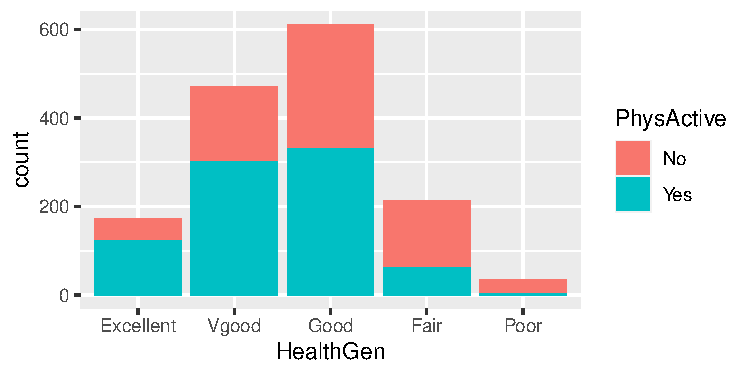
\includegraphics[width=\maxwidth]{figure/unnamed-chunk-3-1} 

\end{knitrout}
\vspace{10pt}

\begin{knitrout}
\definecolor{shadecolor}{rgb}{0.969, 0.969, 0.969}\color{fgcolor}
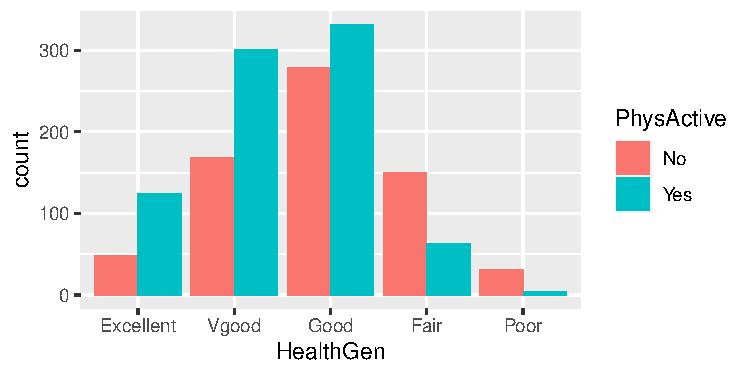
\includegraphics[width=\maxwidth]{figure/unnamed-chunk-4-1} 

\end{knitrout}
\vspace{10pt}

\begin{knitrout}
\definecolor{shadecolor}{rgb}{0.969, 0.969, 0.969}\color{fgcolor}
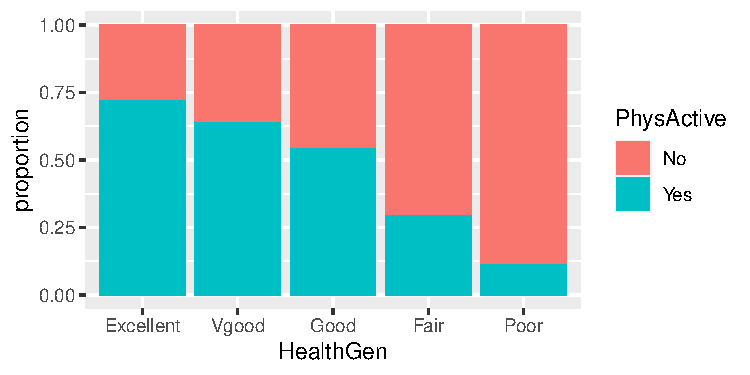
\includegraphics[width=\maxwidth]{figure/unnamed-chunk-5-1} 

\end{knitrout}

\end{document}
